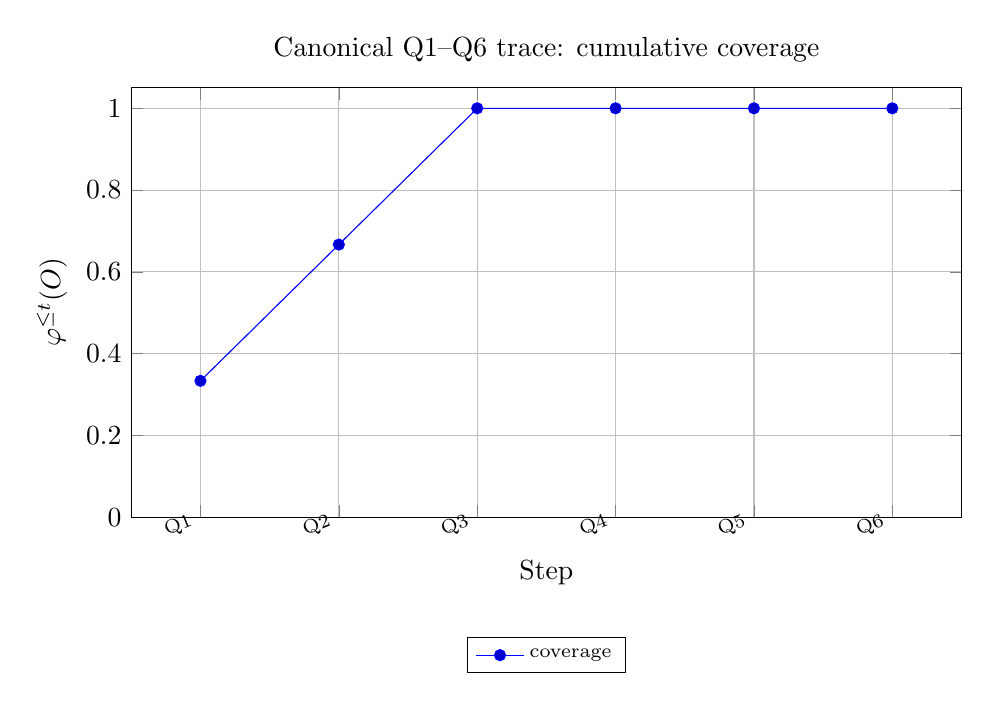
\begin{tikzpicture}
\begin{axis}[width=\linewidth,
height=0.58\linewidth,
title={Canonical Q1--Q6 trace: cumulative coverage},
xlabel={Step},
ylabel={$\varphi^{\leq t}(O)$},
grid=major,
legend style={font=\scriptsize,at={(0.5,-0.28)},anchor=north,legend columns=1},
xtick={1,2,3,4,5,6},
xticklabels={{Q1},{Q2},{Q3},{Q4},{Q5},{Q6}},
x tick label style={rotate=22,anchor=east,font=\scriptsize},
ymin=0,
ymax=1.05]
\addplot+[mark=*] coordinates {(1,0.3333333333333333) (2,0.6666666666666666) (3,1.0) (4,1.0) (5,1.0) (6,1.0)};
\addlegendentry{coverage}
\end{axis}
\end{tikzpicture}
